\colorlet{challengecolour}{uofgcobalt}
\colorlet{challengemapcolour}{challengecolour!40}

\colorlet{respcolour}{uofgthistle}

\begin{tikzpicture}
	\node (circuit) at (0,0) {\resizebox{4cm}{!}{
		\begin{circuitikz}
%			\draw (0,0) to[short, o-*] (1,0) to [cuteopenswitchshape] (2,0) to[tDo] (3,0);
			
			% main block
			
			\node [cuteopenswitchshape] (sw1) at (2,2) {};
			\draw (sw1.out) to[tDo] ++(1,0) to[short, -*] ++(1,0) -- ++(0,-3);
			
			\node [cuteclosedswitchshape] (sw2) at ($(sw1) - (0,1)$) {};
			\draw (sw2.out) to[tDo] ++(1,0) to[short, -*] ++(1,0);
			
			\node [cuteclosedswitchshape] (sw3) at ($(sw2) - (0,1)$) {};
			\draw (sw3.out) to[tDo] ++(1,0) to[short, -*] ++(1,0);
			
			\node [cuteopenswitchshape] (sw4) at ($(sw3) - (0,1)$) {};
			\draw (sw4.out) to[tDo] ++(1,0) to[short, -*] ++(1,0);
			
			% routing to main block
			\draw (sw1.in) -- ++(-1, 0) -- ++(0,-3) -- ++(1,0);
			\draw (sw2.in) to[short,-*] ++(-1, 0);
			\draw (sw3.in) to[short,-*] ++(-1, 0);
			
			% dashed block
			
			\draw ($(sw1.out) + (2,0)$) -- ++(0.5,0);
			\draw[dashed] ($(sw1.out) + (2.5,0)$) -- ++(1,0);
			\draw ($(sw1.out) + (3.5,0)$) -- ++(0.5,0);
			
			\draw ($(sw2.out) + (2,0)$) -- ++(0.5,0);
			\draw[dashed] ($(sw2.out) + (2.5,0)$) -- ++(1,0);
			\draw ($(sw2.out) + (3.5,0)$) to[short, -*] ++(0.5,0);
			
			\draw ($(sw3.out) + (2,0)$) -- ++(0.5,0);
			\draw[dashed] ($(sw3.out) + (2.5,0)$) -- ++(1,0);
			\draw ($(sw3.out) + (3.5,0)$) to[short, -*] ++(0.5,0);
			
			\draw ($(sw4.out) + (2,0)$) -- ++(0.5,0);
			\draw[dashed] ($(sw4.out) + (2.5,0)$) -- ++(1,0);
			\draw ($(sw4.out) + (3.5,0)$) -- ++(0.5,0) -- ++(0,3);
			
			%output
			\draw ($(sw3.out) + (4,0.5)$) to[short,*-] ++(1,0);
			
			%input
			\draw ($(sw3.in) + (-1,0.5)$) to[short,*-] ++(-1,0);
			
		\end{circuitikz}
	}};

	% Challenge
	\node[text=challengecolour,font=\scriptsize] (cval) at ($(circuit) + (0,1.3)$) {\texttt{0110\hspace{0.15em}1101\hspace{0.15em}....}};
	\node[text=challengecolour,font=\scriptsize] (ctext) at ($(cval) + (-0.2,0.25)$) {Challenge: $n$ bits};
	
	\node (boxstart) at ($(cval) - (1.1,-0.2)$) {};
	\draw[color=challengecolour, thick] (boxstart) -- ++(0,-0.4) -- ++ (2.2,0) -- ++ (0, 0.28);
	\draw[color=challengecolour, thick] ($(boxstart) + (0.75,-0.4)$) -- ++(0,0.1);
	\draw[color=challengecolour, thick] ($(boxstart) + (1.45,-0.4)$) -- ++(0,0.1);
	
	% Challenge map
	\draw[color=challengemapcolour, densely dotted, thick] ($(boxstart) + (0,-0.4)$) -- ++(-0.33,-0.4);
	\draw[color=challengemapcolour, densely dotted, thick] ($(boxstart) + (0.75,-0.4)$) -- ++(0.8,-0.4);
	\draw[color=challengemapcolour!50, densely dotted, thick] ($(boxstart) + (1.45,-0.4)$) -- ++(0.3,-0.2);
	\draw[color=challengemapcolour, densely dotted, thick] ($(boxstart) + (2.2,-0.4)$) -- ++(0.35,-0.4);
	
	% Resp graph
%	\node (rg) at (3,1) {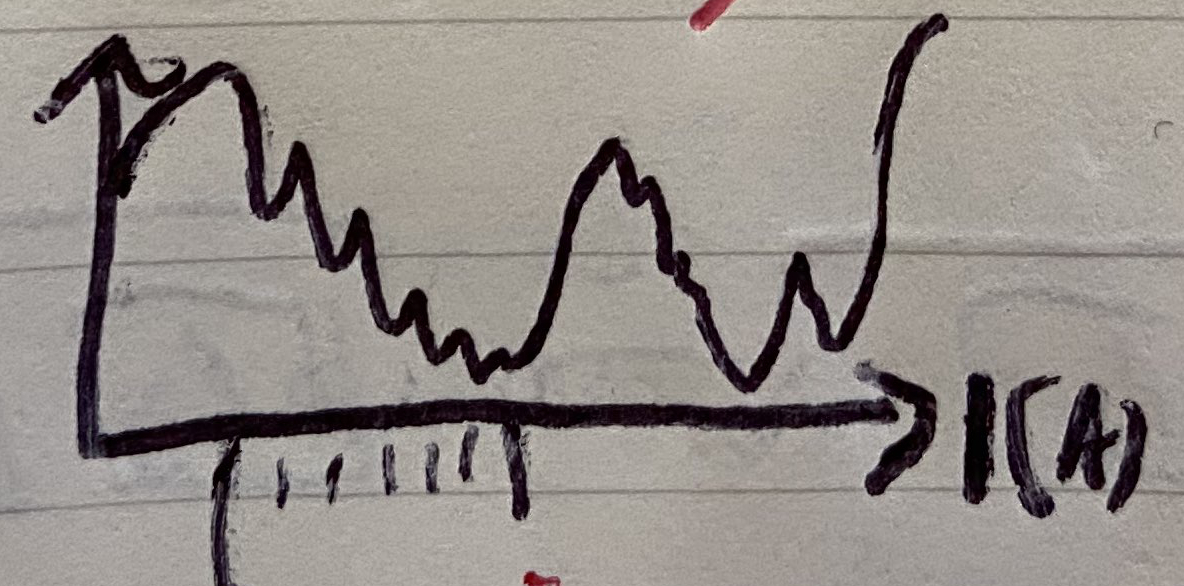
\includegraphics[keepaspectratio,width=2cm]{images/ivchar-draft}};
	\node (rg) at (4,0.5) {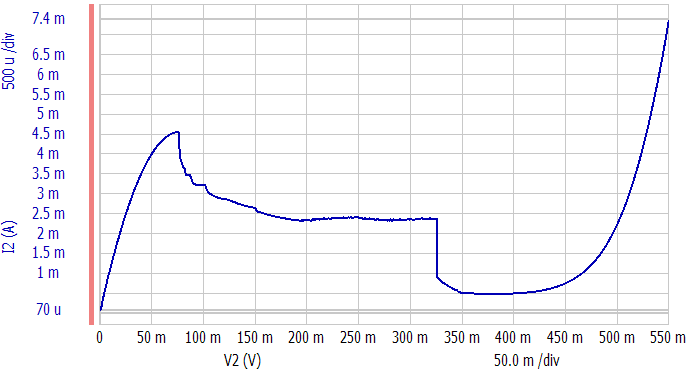
\includegraphics[keepaspectratio,width=3.5cm]{images/VI-png}};
	
	% Response
	\node[text=respcolour] (rval) at ($(rg) + (1,-1.3)$) {\texttt{u8}||\texttt{u8}||...||\texttt{u8}};
	\node[text=respcolour,font=\scriptsize] (rtext) at ($(rval) - (0,0.26)$) {Response: $m$ bits};
	
	\draw[color=respcolour, dashed] ($([xshift=-25]rg.south) + (0,0.4)$) -- ($([xshift=-25]rg.south) + (0,1.3)$);
	\draw[color=respcolour, dashed] ($([xshift=14]rg.south) + (0,0.4)$) -- ($([xshift=14]rg.south) + (0,1.3)$);
	\draw[color=respcolour, <->] ($([xshift=-25]rg.south) + (0,0.7)$) -- ($([xshift=14]rg.south) + (0,0.7)$);
	
	\draw[->, color=respcolour] ($(rg) - (2.45,0.5)$) to[out=90, in=180] (rg.west);
	
	\draw[->, color=respcolour] ($([xshift=14]rg.south) + (0,0.4)$) to[out=-90, in=90] ([xshift=20,yshift=5]rval);
	\draw[->, color=respcolour] ($([xshift=-25]rg.south) + (0,0.7)$) to[out=-90, in=100] ([xshift=-20,yshift=5]rval);
\end{tikzpicture}